\begin{figure}[ht]
    \centering
    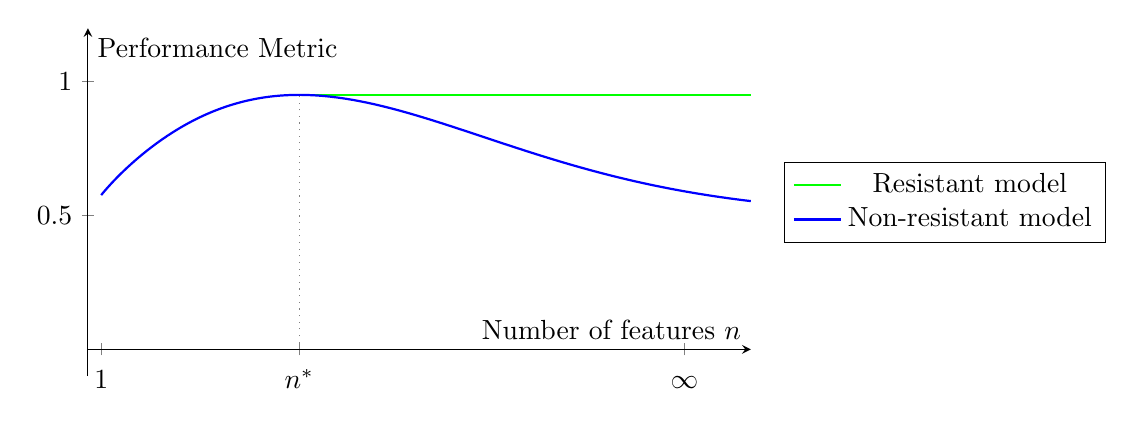
\begin{tikzpicture}
        \begin{axis}[
                axis lines=middle,
                xlabel={Number of features $n$},
                ylabel={Performance Metric},
                samples=1000, domain=1:50,
                xmin=0, xmax=50, ymin=-0.1, ymax=1.2,
                xtick={1,15.94,45},
                xticklabels={\strut 1, \strut $n^*$, \strut $\infty$},
                % extra x ticks={1,18,45},
                %extra x tick labels={1, $n^*$, $n\to\infty$},
                ytick={0,0.5,1},
                width=10cm, height=6cm,
                legend style={at={(1.05,0.5)},anchor=west},
            ]
            \pgfmathsetmacro{\kap}{1.8}
            \pgfmathsetmacro{\lam}{0.04}
            \pgfmathsetmacro{\optimumX}{15.94}
            \pgfmathsetmacro{\optima}{0.5 + 14*(\lam*\kap*(\lam*\optimumX)^(\kap-1)*exp(-(\lam*\optimumX)^\kap))}
            \addplot[green, thick,restrict x to domain=\optimumX:50]{\optima};
            \addlegendentry{Resistant model}
            \addplot[blue, thick] { 0.5 + 14*( \lam*\kap*(\lam*x)^(\kap-1)*exp( -(\lam*x)^\kap ) )};
            \addlegendentry{Non-resistant model}
            \addplot[gray, dotted, forget plot] coordinates {(\optimumX,0) (\optimumX,\optima)};

        \end{axis}
    \end{tikzpicture}
    \caption{Idealistic curves for model performances determined by selected number of features and the resistance to non-informative features.}
    \label{fig:feature-performance}
\end{figure}